%==========================================================================
\section{Method: Zero-Shot Normalised CP}
\label{sec:method}
The method has three deterministic phases, a confidence-adjusted score, an
episode-level calibration unit, and a deployed threshold
(Figure~\ref{fig:pipeline}). It holds no trainable parameters and adds no
latency.

\begin{figure*}[t]
\centering
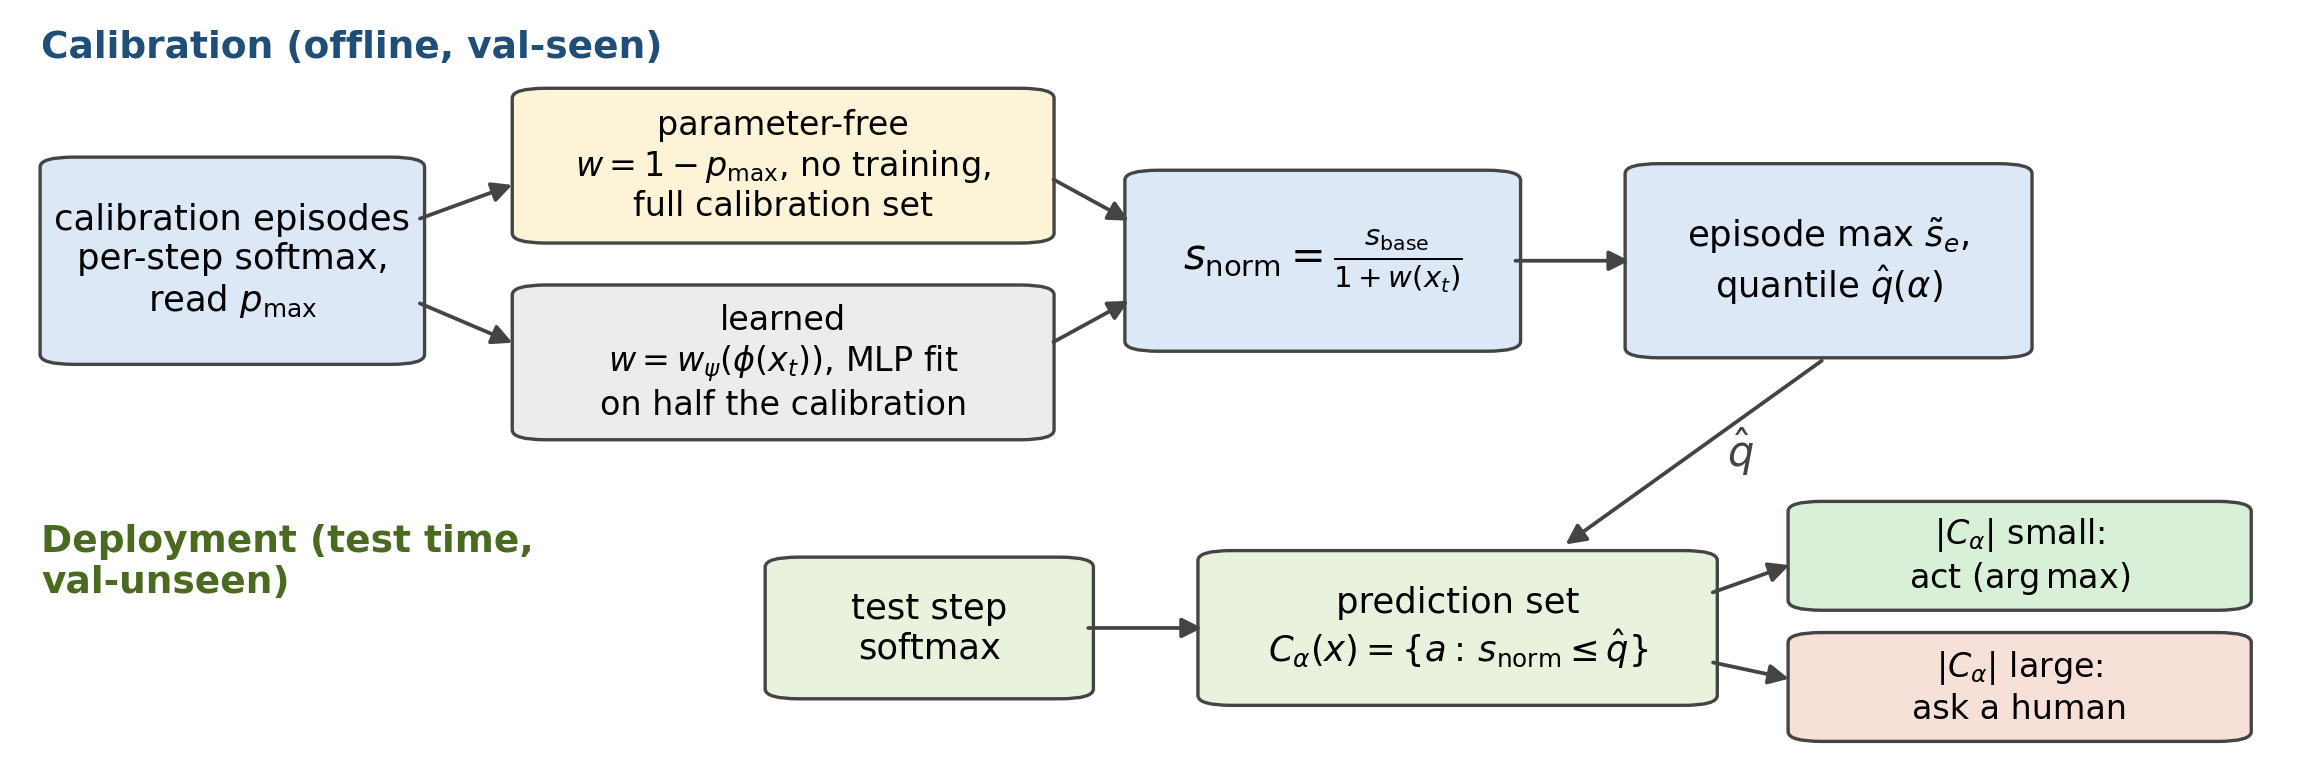
\includegraphics[width=0.8\textwidth]{figures/fig_pipeline.png}
\caption{Overview of the pipeline. \emph{Calibration (offline):} per-step
scores are normalised as $\snorm=\sbase/(1+w(x_t))$ with the parameter-free
weight $w=1-\pmax$ or a learned $w_\psi(\phi(x_t))$
(Section~\ref{ssec:learned}); each episode reduces to its maximum score,
whose corrected quantile gives $\hat q(\alpha)$. \emph{Deployment:} the set
\eqref{eq:set} widens where the policy is uncertain, flagging the step for
a human query.}
\label{fig:pipeline}
\end{figure*}

\subsection{The confidence-adjusted nonconformity score}
\label{ssec:score}
To counter the concentration of Section~\ref{ssec:failure} we rescale any
base score $\sbase \in \{s_{\mathrm{THR}}, s_{\mathrm{APS}},
s_{\mathrm{RAPS}}\}$ of \eqref{eq:thr}--\eqref{eq:raps} by a parameter-free proxy read straight off the policy
confidence $\pmax = \max_a \pi_\theta(a\mid L, x_t, h_t)$,
\begin{equation}
\snorm(x_t, a) \;=\; \frac{\sbase(x_t, a)}{1 + \big(1 - \pmax\big)}
\;=\; \frac{\sbase(x_t, a)}{2 - \pmax}.
\label{eq:snorm}
\end{equation}
The denominator $1 + (1-\pmax)$ is one positive scalar shared by every
candidate at step $t$, so \eqref{eq:snorm} rescales the scores and keeps their
order. On a confident step $\pmax \approx 1$, the denominator goes to $1$ and
$\snorm \approx \sbase$, so easy steps are left alone and the set does not
grow. On an uncertain step $\pmax$ is low, the denominator grows, $\snorm$
shrinks, more candidates pass the threshold, and the set widens where the
robot is confused. The membership test $\snorm(x,a) \leq \hat q$ rewrites
to $\sbase(x,a) \leq \hat q\,(2 - \pmax)$, a base score read against a
confidence-adaptive threshold, and evaluating it costs one subtraction per
step. The set ranges over the valid candidates of $\mathcal{A}_t$
(Section~\ref{sec:problem}), so a masked action is never included.

\subsection{Episode-maximum calibration unit}
\label{ssec:epmax}
Per-step pairs within an episode share $h_t$ and are not exchangeable, so
step-pooled calibration breaks the CP requirement and gives no guarantee on
whole-trajectory survival. We reduce each calibration episode $e$ (steps
$1\dots T_e$, teacher actions $a^*_t$) to a single most-surprising correct
score,
\begin{equation}
\tilde{s}_e \;=\; \max_{t \in \{1,\dots,T_e\}} \snorm(x_{e,t}, a^*_{e,t}),
\label{eq:epmax}
\end{equation}
which restores exchangeability at the episode level and targets simultaneous
coverage over the walk (Theorem~\ref{thm:cov}).

\subsection{Threshold and test-time inference}
\label{ssec:infer}
Given $\alpha$ and $n$ exchangeable calibration episodes, the threshold is
the corrected quantile of the episode-maximum scores,
\begin{equation}
\hat q(\alpha) = \mathrm{Quantile}\Big(\{\tilde s_1,\dots,\tilde s_n\};\,
\tfrac{\lceil(n+1)(1-\alpha)\rceil}{n}\Big).
\label{eq:qhat-ep}
\end{equation}
Because the score is fixed and parameter-free, all $n$ calibration episodes
are exchangeable with the test episode, so there is no train-calibrate split
and $n$ is the full calibration set (Remark~\ref{rem:paramfree}). At test time
the agent extracts $\pmax$ from its softmax and forms
\begin{equation}
C_\alpha(x_t) = \{a \in \mathcal{A}_t : \snorm(x_t, a) \leq \hat q(\alpha)\},
\label{eq:set}
\end{equation}
with the $\arg\max$ action as fallback when the set is empty. There is no
training loop, and Section~\ref{sec:disc} closes the loop by querying an
operator when the set grows.

\subsection{Learned and hybrid weights}
\label{ssec:learned}
The score \eqref{eq:snorm} is one member of a family
$\snorm=\sbase/(1+w(x_t))$, and the guarantee of
Section~\ref{sec:guarantee} holds for every weight fixed before
calibration. Besides the parameter-free $w=1-\pmax$, a learning-based
member sets $w=w_\psi(\phi(x_t))$, a small MLP over softmax statistics fit
on half of the calibration episodes, and a hybrid adds a learned
non-negative residual to the parameter-free floor. Both preserve the
theorem at the cost of a train--calibrate split and a second forward pass
(Remark~\ref{rem:paramfree}), and both match the parameter-free coverage
(Section~\ref{sec:disc}).
